\documentclass[11pt]{article}
\usepackage[paperwidth=12cm, paperheight=18cm, margin=1cm]{geometry}
\usepackage{amsmath, tikz}
\pagestyle{empty}

\begin{document}
\begin{center}
  {\LARGE\bfseries The Birthday Paradox}\\[4pt]
  {\large 23 people are enough for a coin flip}
\end{center}

How many people do you need in a room for a 50\% chance
that two of them share a birthday? Not 183. Just 23.

\section*{Count the ways nobody matches}
\[
  P(\text{no match}) = \prod_{k=0}^{n-1} \frac{365 - k}{365}
  \approx e^{-\frac{n(n-1)}{730}}
\]

\section*{With 23 people}
\[
  P(\text{match}) = 1 - \frac{365!}{342!\;365^{23}} \approx 50.7\%
\]

\begin{center}
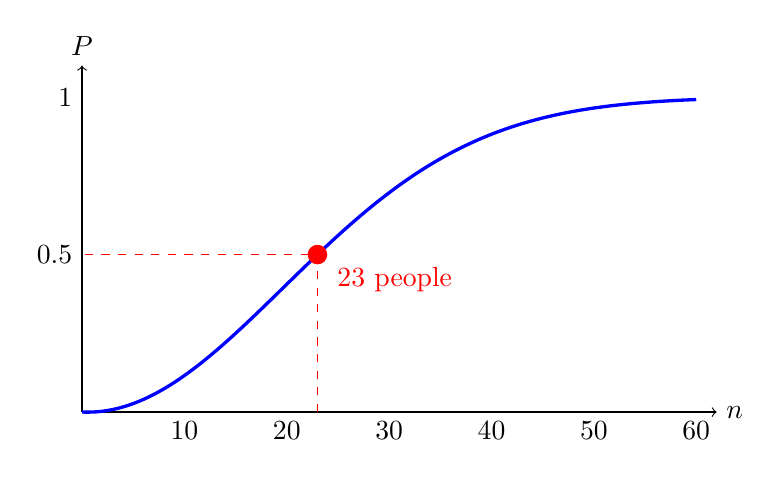
\begin{tikzpicture}[xscale=0.13, yscale=4]
  \draw[->] (0,0) -- (62,0) node[right] {$n$};
  \draw[->] (0,0) -- (0,1.1) node[above] {$P$};
  \foreach \y in {0.5, 1} \node[left] at (0,\y) {\y};
  \foreach \x in {10, 20, 30, 40, 50, 60} \node[below] at (\x,0) {\x};
  \draw[blue, very thick, domain=0:60, samples=120]
    plot (\x, {1 - exp(-\x*(\x-1)/730)});
  \draw[red, dashed] (23,0) -- (23,0.5) -- (0,0.5);
  \node[circle, fill=red, inner sep=2.5pt] at (23,0.5) {};
  \node[red, right] at (24,0.42) {23 people};
\end{tikzpicture}
\end{center}

Why so few? With 23 people there are \(\binom{23}{2} = 253\) pairs,
and every pair is a chance for a match.
\end{document}
